%----------------------------------------------------------------------------------------
%	GENERAL.
%----------------------------------------------------------------------------------------
\clearpage

\section{\label{sec:general}General Spacecraft Environment Description}

\subsection{Low Earth Orbit Regime}

\begin{figure}[h!]
\centering
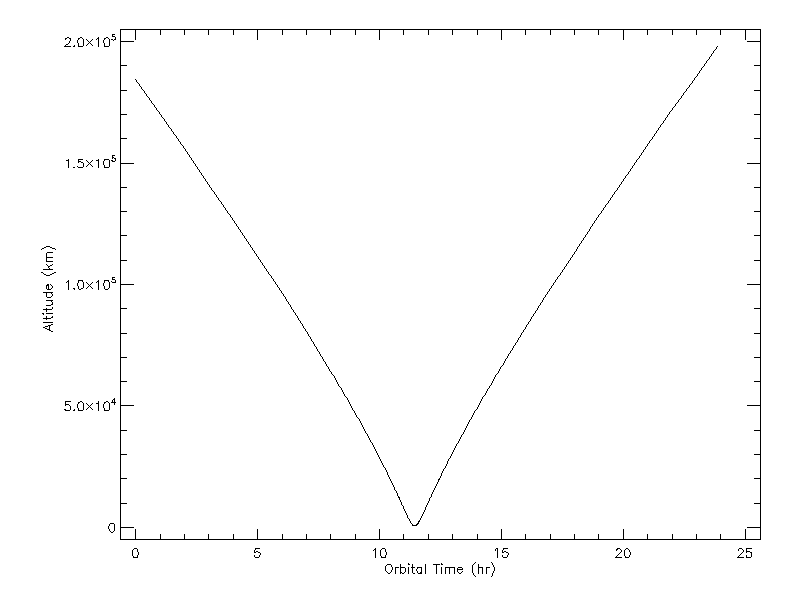
\includegraphics[width=0.7\textwidth]{figures/AltVSTime.png}
\caption{Satellite altitude plotted over time}
\label{AltPlot}
\end{figure}

Figure \ref{AltPlot} shows the variation of the  altitude of Willzyx I with time. Here we can see again that the altitude will only continue to increase, meaning again that the Willzyx I will be leaving Earth's gravitational pull. This can be further confirmed by comparing the escape velocity at Willzyx I perigee with the actual velocity of the spacecraft. Such calculation is done with the following equations:

\begin{equation}
v_{esc}=\sqrt{\frac{2\mu}{r}}=10.66\,km/s
\label{Vesc}
\end{equation}
This is the escape velocity equation. With $\mu$ being the standarg gravitational parameter and r is the distance to the center of mass of Earth in this case. For the velocity of the spacecraft at a certain point, we use:

\begin{equation}
v=\sqrt{\mu(\frac{2}{r}-\frac{1}{a}}=11.18\,km/s
\label{Vsc}
\end{equation}

Using this equation we obtain the velocity of the spacecraft with respect to Earth. $\mu$ and r are the same as in equation \ref{Vesc} and a is the semi-major axis of the hyperbola describing the trajectory.

As we can see, the velocity of the spacecraft is higher than the Earth's escape velocity, confirming that the trajectory is hyperbolic.

We also note from figure \ref{AltPlot} that the spacecraft will be below 2000\,km even if it's for about 2\% of the mission time. This means that we have to take into account the environment in the Low Earth Orbit regime.

\begin{figure}[h!]
\centering
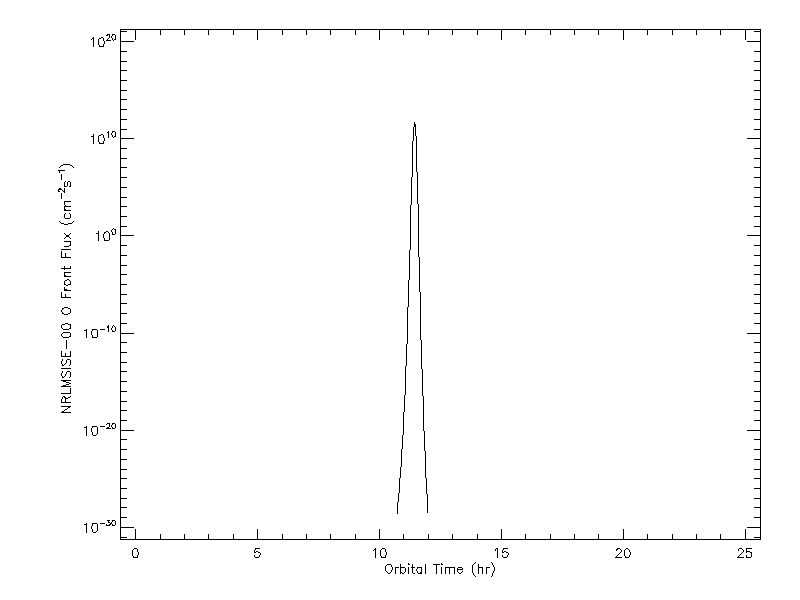
\includegraphics[width=0.7\textwidth]{figures/OxTime.png}
\caption{Frontal flux of atomic oxygen}
\label{Oxygen}
\end{figure}

Figure \ref{Oxygen} shows the frontal flux of oxygen during the flyby of Willzyx I during the time spent in the LEO regime. The peak will be reached at the perigee, with values in the order of $10^{14}$ oxygen molecules$/cm^2$. This atomic oxygen could cause degradation on the spacecraft walls and shielding which given enough time could impair the functionality of the spacecraft. Given the very little time that the spacecraft will spend in the LEO regime, and in particular in the altitudes close to the perigee, no significant degradation of the shielding is expected.

\subsection{Medium Earth Orbit regime}

During the flyby of Willzyx I over the Earth, it will pass by the Medium Earth Orbit regime (between 2000\,km and 36000\,km). In this region, the concentration of molecules from Earth's atmosphere like oxygen is extremely low and can be completely disregarded. The main concerns would be radiation and plasma.

The radiation environment in this region is comprised of electromagnetic radiation and high energy particles trapped in the Van Allen belts, they extend between 640 and 58\,000\,km. The particles trapped in these belts range from electrons and protons to other heavier ions. Other radiation sources in this region are the solar wind and Cosmic rays. The radiation present in this region can be harmful to electronic components, with the most common problem that emerges being the single even upsets in the memory of the spacecraft, also known as bit flips.

The plasma present in this region can produce electrostatic charging on different components of the spacecraft. Some of the possible problems include: The change of the ground electric potential of the spacecraft which could lead to calibrations issues, in many other cases this charging can be uneven along the spacecraft, which can cause interference in the most sensitive sensors and in some cases it could cause a spark within the components. 

\subsection{High Earth Orbit and Beyond}

When the spacecraft is farther away than 36\,000\,km it enters the High Earth orbit. Here, far away from the inner Van Allen radiation belts, the spacecraft will pass through the outer radiation belt. This belt has particles with higher energy and it's more variable in it's extension but not exceeding 60\,000\,km if altitude. Similar considerations as the for the MEO regime must be taken. Particles in this region are also more sparse, lowering the probability of interaction with the spacecraft.
